\documentclass[accentcolor=tud9d,colorbacktitle,inverttitle,landscape,german,presentation,t]{tudbeamer}
\usepackage{ngerman}
\usepackage[T1]{fontenc}
\usepackage[latin1]{inputenc}
\usepackage{helvet}
\usepackage{graphicx}
\usepackage{picins}


\begin{document}

	% Titel
	\title{Instant Message Whispering via Covert Channels}
	\subtitle{Gruppe 35\\Simon Bunten, Simon Kadel, Martin Oehler, Arne St�hlmeyer}
	
 	% Fu�zeile
	\author{Simon Bunten, Gruppe 35}
	\date{22. November 2013}
	\logo{
\includegraphics{../Bilder/tklogo.jpg}}

\begin{titleframe}
	\begin{figure}
	\centering
	
\includegraphics[scale=.55]{../Bilder/InstantMessenger.jpg}
	\end{figure}
\end{titleframe}

\begin{frame}
	\frametitle{Einf�hrung}
	
	\begin{minipage}{.55\linewidth}
	Verstecktes Instant Messaging
	\begin{itemize}
		\item Vermeiden von Entdeckung, Abh�ren und Abfangen
		\item Senden von Nachrichten durch Firewalls
	\end{itemize}	
	
	\end{minipage}
	\hfill
	\begin{minipage}{.4\linewidth}
	{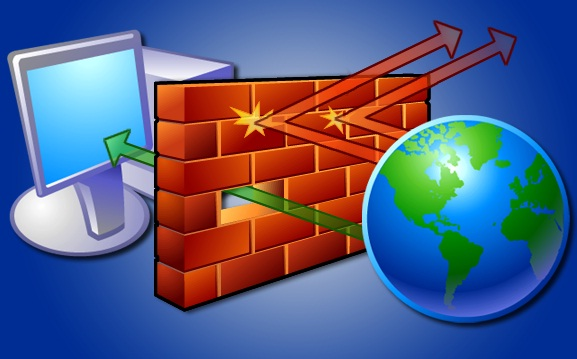
\includegraphics[scale=.3]{../Bilder/Firewall.jpg}}
	\end{minipage}
	
	\begin{description}
		\item {}
		\item <2>[Kryptographie] Verschl�sselt die Daten, Kanal bleibt sichtbar
		\item<2>[Covert Channels] Versteckt den Kanal
	\end{description}
	
\end{frame}

\begin{frame}

	\frametitle{Projektbeschreibung}
	Programmieren einer Bibliothek f�r Covert Channels
	\begin{itemize}
		\item <2->�ffnet und verwendet Covert Channels
		\item <3->Implementierung eines Frameworks
		\item <4->konkrete Covert Channels als Plugin
		\item <5->Ver�ffentlichung als Open Source
		\item <6->Beispielumsetzung im Stil eines Instant Messagers
	\end{itemize}
	\begin{center}
	%\parpic[r]{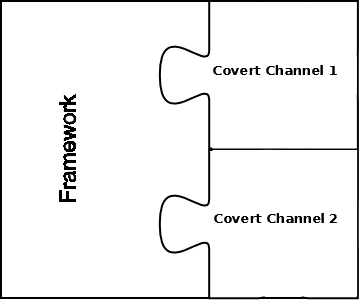
\includegraphics[scale=0.25]{Bilder/framework-puzzle.png}}
	\end{center}

\end{frame}

\begin{frame}

	\frametitle{QS-Ziele und ihre Sichherstellung}
	\begin{itemize}
		\item <1->\textbf{Modularit�t} \\
		\only<2>
		{\begin{itemize}
			\item Modulares Design des Framework
			\item Feste, dokumentierte Modulschnittstellen
		\end{itemize}}
		\item <3->\textbf{Zuverl�ssigkeit} \\
		\only<4>
		{\begin{itemize}
			\item automatisierte Tests
		\end{itemize}}
		\item <5->\textbf{Testbarkeit}	\\
		\only<6>
		{\begin{itemize}
			\item klare, getrennte Verantwortlichkeiten
			\item Isolierbarkeit durch Module
		\end{itemize}}
	\end{itemize}

\end{frame}

\begin{frame}
	\frametitle{Zeitaufwand}
	\begin{center}
		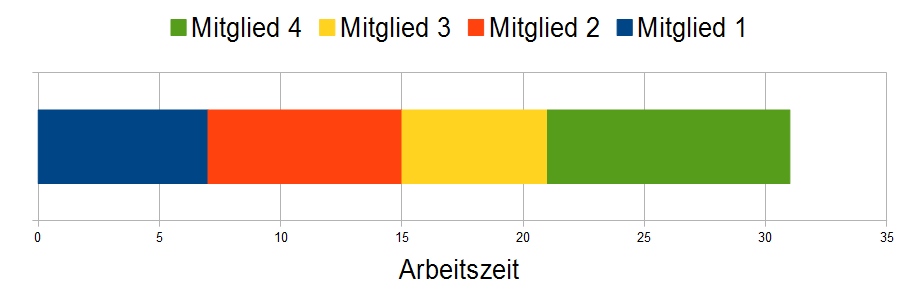
\includegraphics[scale=0.5]{../Bilder/zeitsummen2.PNG} \newline
	\end{center}

\end{frame}

\begin{frame}
\frametitle{Zeitmanagement}
	\begin{center}
		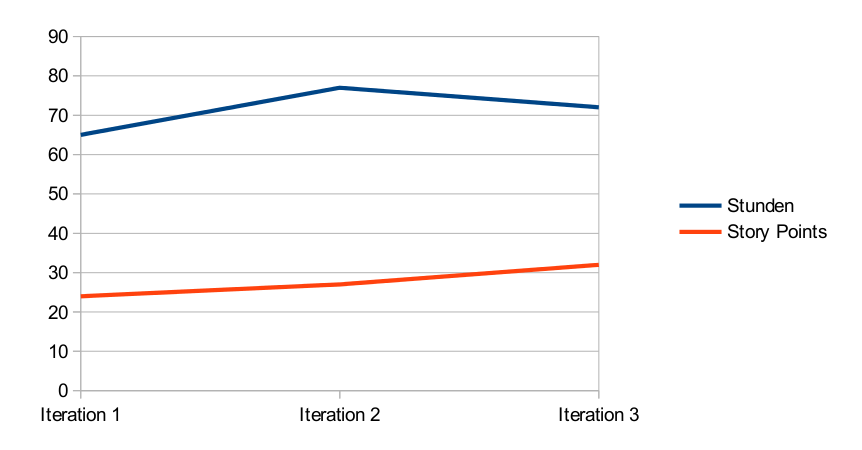
\includegraphics[scale=.35]{../Bilder/stunden_storypoints.png}
	\end{center}

\end{frame}

\begin{frame}
\frametitle{Zeitmanagement}
	\begin{center}
		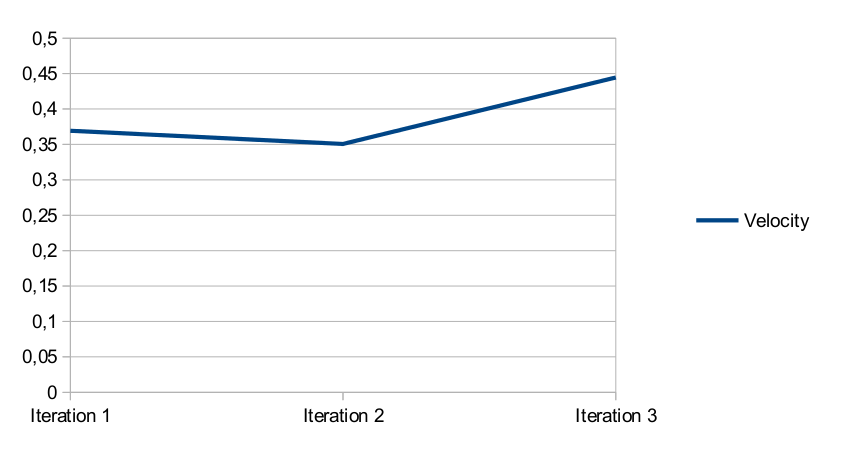
\includegraphics[scale=.35]{../Bilder/velocity.png}
	\end{center}

\end{frame}

\begin{frame}
\frametitle{Zusammenfassung}
	\begin{itemize}
		\item Entwicklung einer Bibliothek f�r die Kommunikation �ber Covert Channels
		\item Trennung von Framework und Implementation der Covert Channels
		\item Modularer Aufbau erleichtert Erweiterungen
		\item Umsetzung in einem Instant Messager als Beispielanwendung
		\item Open-Source-Ver�ffentlichung setzt hohe Qualit�tsanspr�che
	\end{itemize}
\end{frame}


\end{document}